\chapter{Estudio del Problema Singular}
{\label{cap.singular}}

El presente capítulo contiene el resultado original de este Trabajo de Diploma, que consiste en el análisis de un operador diferencial con un coeficiente singular. Como hemos mencionado, el desarrollo asintótico (\ref{eq.heat.expansion})
es válido para operadores diferenciales con coeficientes suaves. En efecto,
mostraremos a continuación que la presencia de una singularidad puede
conducir a un desarrollo asintótico de la traza del heat-kernel que no con-
tiene exclusivamente potencias semi-enteras de $T$, contradiciendo el resultado \ref{eq.heat.expansion}. Veremos que
en el caso del operador singular que hemos analizado el desarrollo del heat-kernel contiene términos $\log T$.


\section{El Operador Singular}


En está sección se estudiará el siguiente operador diferencial definido sobre funciones $\phi (x)\in \mathbb{L} ^2 [0,L]$,
\begin{equation}
\begin{aligned}
    A \phi (x) &= - \partial ^2 _x  \phi(x) + \frac{\alpha}{x} \phi(x) \\[5pt]
    \phi(0) &= \phi(L) = 0 \, .
\end{aligned}
\label{operador}
\end{equation}
Por simplicidad, se analizaran condiciones Dirichlet en ambos extremos.  El parámetro $\alpha \in \mathbb{R _{+}}$ caracteriza la singularidad en el origen.
Los autovalores están dados por la ecuación 
\begin{equation}
\begin{aligned}
    A  \phi (x)  &=   \lambda ^2 \phi (x) \\[5pt]
    \lambda ^2 \ &\in \ \mathbb{R}  
    \, ,
\end{aligned}
\label{eq.aut.sin}
\end{equation}
las autofunciones en términos de dos soluciones linealmente independientes $\phi _1 (x), \phi _2 (x)$ pueden escribirse
\begin{align}
\label{eq.phi}
&
    \phi (x) =
\\
&
	    C _1
    	\underbrace{
				     \ e ^{-i \lambda x} \ x \ 
				     F _{1} ^{1} 
				     		\left(  
				     			1 - \frac{i \alpha}
				     			{2\lambda}
				     		,2,2 i \lambda x \right) 
				     } _ {\phi_1} + 
      C _2 
      \underbrace{ 
      			   \ e^{-i \lambda x } \ x \ 
      			   U 
      			   	\left( 
      			   		1- \frac{i \alpha}{2 \lambda}
      			   		,2,2 i \lambda x \right) } _{\phi_2} 
    \, ,
\nonumber
\end{align}
donde $F _1 ^1(a,b,z)$ y $ U(a,b,z)$ son las soluciones LI de la ecuación {\mbox{hypergeométrica} }
\begin{equation}
    z \ \partial ^2 _z \ \psi (a,b,z) + (b-z) \
    \partial _z \psi (a,b,z)
    -a \ \psi (a,b,z) = 0 \, .
\end{equation}
las cuales están dadas por \cite{Abramowitz:hyper}
\begin{align}
	U(a,b,z) = &\frac{1}{\Gamma (a)} 
	\int _0 ^{\infty} e ^{-zt}
	t ^{a-1}
	(1+t) ^{b-a-1}
	dt \\
	& {\rm si \ } Re (b) > Re(a) 
	\nonumber
	\\[5pt]
	F _1 ^1 (a,b,z) =& \sum _ {k=0} ^{\infty} 
	\frac{(a) _k}{(b) _k} 
	\frac{z ^k}{k!} 
	\, ,
\end{align}
donde $(.) _n$ es el símbolo de Pochhammer.
Si se cumple que  $a=-m,b \neq -n$ donde $ m,n \in \mathbb{N}$, $F _1 ^1 (a,b,z)$ es un polinomio en $z$ y $U(a,b,z)$ es linealmente dependiente con $F _1 ^1 (a,b,z)$, en tal caso se usa $z^{1-b} M(a+1,-b,2-b,z)$ como segunda solución LI.


Las constantes $C_1,C_2$ están sujetas al vínculo impuesto por las condiciones de contorno.
Para imponer las condiciones de contorno, primeramente desarrollamos $\phi (x)$ cerca de $x \simeq 0$ 
\begin{align}
\phi  ( x ) &=
C _1  x  + 
C _2 \ x 
\left( 
\frac{1}{  \alpha x  \Gamma ( - \frac{i \alpha}{2  \lambda}  )   }  +
\frac{\log (x) }{\Gamma ( - \frac{ i \alpha}{2 \lambda} ) } + \mathscr{C} \right) + O(x ^2)
	\nonumber
\\[10pt]
\mathscr{C} &= 
\frac{
-1 + 2 \gamma + \log ( 2  i \lambda ) + \psi (1 - \frac{i \alpha}{2 \lambda})
}
{\Gamma (\frac{i \alpha}{2 \lambda})}
\, ,
\label{eq.scat}
\end{align}
Un detalle a tener en cuenta es que si sucede que $\Gamma ( \frac{i \alpha}{2 \lambda}  ) \rightarrow \infty$ entonces $\phi (0) = 0$ indepenientemente de $C _1$ y $C _2$, el problema radica en que no puede simplemente hacerse el reemplazo $\lambda \rightarrow  \frac{i \alpha }{ n } $ con $n=1,2,3 \dots$ en \eqref{eq.phi}. 

Para tratar este caso se escribe el autovalor $\lambda ^2 = - \frac{\alpha ^2}{4 n ^2}$ con $n \in \mathbb{R _+}$ en la ecuación \eqref{eq.aut.sin} cuyas soluciones están dadas por
\begin{align}
& \nonumber 
	\phi (x)     =
\\ &        
	    C _1
    	\underbrace{
				     \ e ^{- \frac{x \alpha}{2n}} \ x \ 
				     F _{1} ^{1}
				     \left( 1+n,2, \frac{x \alpha}{n} \right) 
				     } _ {\phi_1} 				     
				     + 
      C _2 
      \underbrace{ 
      			   \ e^{- \frac{x \alpha}{2n}} \ x \ 
      			   U 
      			   \left( 1+n,2, \frac{x \alpha}{n} \right)
      			   } _{\phi_2} 
    \, ,
\label{eq.phi.2}
\end{align}
utilizando esta solución se obtiene para $\phi (x) $ cerca de $x \simeq 0$ 
\begin{align}
\nonumber
	\phi (x) 
&=
	C _1 x 
	\left(1 + \frac{(1+n) \alpha x}{2 n } \right)
	+ C _2 x
	\left(
	\frac{1}{\alpha \Gamma (n) x } + \frac{\log (x)}{\Gamma (n)} +\mathscr{C}
	\right)
	+ O(x)
\\
\mathscr{C} 
&=
\frac{\psi (1+n) + \log \left( \frac{\alpha}{n} \right) -1 + 2 \gamma}{\Gamma (n)}
\, ,
\end{align}
lo cual implica $C _2 = 0$. Con lo cual el problema de energías negativas queda determinado por los ceros de.
\begin{equation}
	F _1 ^1 
	\left(
		1+n,2, \frac{L \alpha}{n}
		\right) = 0
\, ,		
\end{equation}
con lo cual el autovalor queda determinado por $\lambda ^2 = - \frac{\alpha ^2}{4 n ^2}$ donde \mbox{$n \in \mathbb{N}$}.


Para los cálculos que nos interesan solo se utilizarán los autovalores $\lambda ^2 >0$. 

Del desarrollo \ref{eq.scat} se ve que la condición de contorno en $x=0$ fija $C _2 =0$. 
Imponiendo entonces la condición de contorno $\phi (L)=0$ se obtiene que los autovalores positivos $\lambda ^2$ están dados por las soluciones de
\begin{equation}
F _1 ^1 \left(1-\frac{i \alpha}{2 \lambda},2,2 i \lambda L \right)  = 0
	\, .
\label{eq.1}
\end{equation}
En la figura (\ref{fig:funcion}) se encuentra graficado
\mbox{$ | F _1 ^1 (1-\frac{i \alpha}{2 \lambda},2,2 i \lambda L) | ^2 $} para $\alpha=1, \ L=1$. Las intersecciones con el eje horizontal indican los autovalores positivos del espectro del operador singular.


\begin{figure}[h!]
\centering
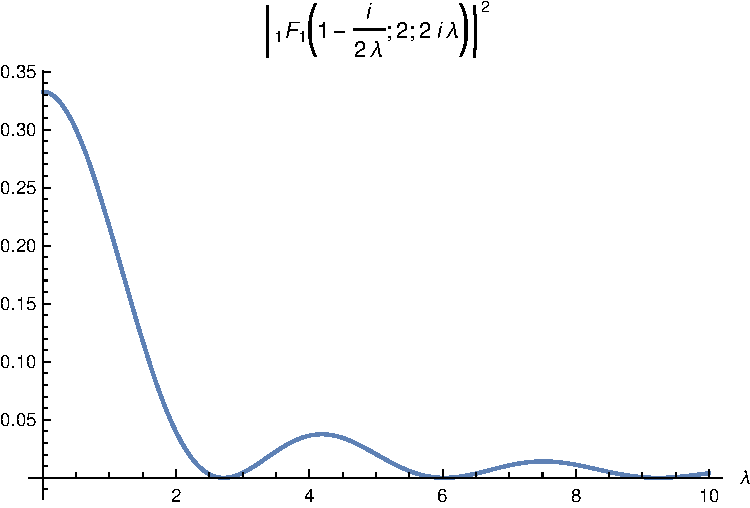
\includegraphics[scale=0.7]{Funcion.pdf}
\caption{En esta imagen se pueden ver los primeros ceros de la función $| F _1 ^1 (1+\frac{ \alpha}{2 i \lambda},2,2 i \lambda L) | ^2$ para $\alpha=1$ y $L=1$, los cuales representan a los primeros autovalores del operador $A$.}
\label{fig:funcion}
\end{figure}


Para calcular $\zeta(s)$ se utilizará el desarrollo asintótico de la funcion $F _1 ^1 (a,b,z)$ a $z \rightarrow \infty$ \cite{Abramowitz:hyper},
\begin{equation}
\begin{aligned}
    F _1 ^1 (a,b,z) &= \Gamma (b) 
    \left(
    \frac{e^z z ^{a-b} }{\Gamma(a)}  S_1 (z) + \frac{(-z) ^{ -a}}{ \Gamma(b-a)} 
    S_2 (z)
    \right) \\[5pt]
    S _1 (z) &= \sum _{n=0} ^{\infty} \frac{(b-a) _n (1-a) _n}{n!} z ^{-n} \\[5pt]
    S _2 (z) &= \sum _{n=0} ^{\infty} \frac{(a) _n (1+a-b) _n}{n!} (-z) ^{-n}     
		\, ,
\end{aligned}
\label{eq.aprox}
\end{equation}
aquí $S_1$ y $S _2$ representan el desarrollo a todo orden.
Utilizando este desarrollo $F _1 ^1 \left(1+  \frac{  \alpha}{2 i \lambda} ,2 ,2 i \lambda L  \right)$ queda determinada por
\begin{align}
\label{eq.completa}
	F _1 ^1 \left(1+  \frac{  \alpha}{2 i \lambda} ,2 ,2 i \lambda L  \right) 
&	
	\sim
    \frac{i e ^{ \frac{\pi \alpha }{4 \lambda}  } }{2 \lambda L}
    \left(
    \frac{e ^{   \frac{ i \alpha}{2 \lambda}  \log (2 \lambda L) }}               {\Gamma(1+\frac{i \alpha}{2 \lambda})} S _2 ( \lambda )-
    \frac{e ^{-  \frac{i \alpha}{2 \lambda}  \log (2 \lambda L) } e ^{2 i \lambda L} }{\Gamma(1-\frac{i \alpha}{2 \lambda})} 
    S _1 ( \lambda )
    \right) 
\nonumber
\\[5pt]
&
    =  i  \frac{e ^{ \frac{\pi \alpha }{4 \lambda}  } }{2 \lambda L}     M (\lambda) 
    \, .
\end{align}
Donde $S _{1,2}$ están expresados en la sección \ref{sec.sig.polos}.
Dado que $M( \lambda)$ posee los mismos ceros que $F _1 ^1 \left(1+  \frac{  \alpha}{2 i \lambda} ,2 ,2 i \lambda L  \right)$ se puede utilizar tanto $M$ como $F$ para estudiar $\zeta (s)$.


En las siguientes dos secciones \ref{seq.2.asin} y \ref{seq.2.com} se utilizará $M ( \lambda )$ al orden mas bajo (lo que corresponde a tomar $S _1 (\lambda) = S _2 ( \lambda )= 1$) para estudiar el polo de $\zeta \left( - \frac{1}{2} \right)$. En la sección \ref{sec.sig.polos} se tendrán en cuenta $S _1 (\lambda)$ y $S _2 ( \lambda )$ en $M ( \lambda)$ para estudiar la estructura de polos en la region ${\rm Re }(s) \geq - \frac{1}{2}$.
Luego finalmente en la sección \ref{sec.regular} se utilizará el desarrollo completo \eqref{eq.completa} para estudiar la parte finita de $\zeta \left( - \frac{1}{2} \right)$.

\section{Cálculo Asintótico de los autovalores}\label{seq.2.asin}

En esta sección seguiremos el procedimiento descrito en \ref{seq.asin} para estudiar la estructura de polos de $\zeta (s)$: calcularemos el desarrollo asintótico de grandes autovalores, que luego será utilizado para determinar los residuos en los primeros polos $s= \frac{1}{2}$ y $s= - \frac{1}{2}$.



Es conveniente definir las variables adimensionales: $\rho _n = \lambda _nL $ y $\beta = \alpha L$. Luego en vez de utilizar $M (\rho _n)$ definida en (\ref{eq.completa}) se trabajará con la función $N (\rho _n)$ definida de la forma
\begin{align}
\label{eq.otro.mu}
\nonumber
N (\rho _n) &=
e ^{\frac{i \beta }{\rho _n} \log(2 \rho _n) }
\Gamma \left( 1 + \frac{ \beta}{2 i \rho _n} \right)
M (\rho _n) \\ 
&=  
e ^{\frac{i \beta }{\rho _n} \log(2 \rho _n) }
\frac{\Gamma \left(1 + \frac{ \beta}{2 i \rho _n} \right)}
	{\Gamma \left(1 - \frac{ \beta}{2 i \rho _n} \right)}
- e ^{2 i \rho _n}
\, .
\end{align}
En el limite de $\rho _n \rightarrow \infty$ se obtiene
\begin{equation}
    N(\rho _n  \rightarrow \infty) = 
	1 - e ^{2 i \rho _n}
		\, ,
\end{equation}
de aquí se puede ver que los ceros de $N ( \rho ) $ cumplen la condición
\begin{align}
\label{eq.mu2}
    &\rho _n = n \pi + \epsilon _n \\[5pt]
\label{eq.mu2.limite}
	&\lim \limits _{n \rightarrow{0}} \epsilon _n  = 0
		\, .
\end{align}
Utilizando las ecuaciones (\ref{eq.mu2}) y \eqref{eq.mu2.limite} en el desarrollo (\ref{eq.otro.mu}) se obtiene una ecuación para $\epsilon _n$
\begin{equation}
	e ^{ i \frac{\beta}{ \rho _n} \log (2 \rho _n)}     
    \frac{\Gamma(1 + \frac{ \beta}{2  i \rho _n} ) }
    {\Gamma(1 -  \frac{ \beta}{2  i \rho _n} )} =    
    e ^{2 i \epsilon _n }
    	\, .
\label{eq.a.desarrollar}
\end{equation}
Utilizando $ \lim \limits_{\rho _n \rightarrow \infty} \frac{\log (2 \rho _n)}{2 \rho _n } \rightarrow 0$ se puede representar (\ref{eq.a.desarrollar}) por su desarrollo en serie en los límites $ \rho _n \rightarrow \infty $ y $\epsilon _n \rightarrow 0$,
\begin{equation}
    \left(
    \sum _{p = 0} ^{\infty} \frac{ \left( i \frac{\beta}{ \rho _n } \log(2 \rho _n ) \right) ^p }{p!}
    \right)
    \left(
	\sum _{q = 0} ^{\infty} \frac{a _q}{\rho _n ^q}
	\right)
    =
    \left(
    \sum _{l = 0} ^{\infty} \frac{( 2 i \epsilon _n)^l}{l !}
    \right)
    	\, .
\end{equation}
A partir de esta ecuación puede verse que el orden dominante de $\epsilon _n$ está determinado por
\begin{equation}
\left( 1 + \frac{i \beta}{ \rho _n} \log ( 2 \rho _n) \right) 
\left(1 + \frac{i  \gamma \beta}{ \rho _n} \right)  =
(1 + 2 i \epsilon _n) \, ,
\end{equation}
resolviendo asintóticamente la ecuación anterior se obtiene $\epsilon _n$
\begin{equation}\label{anterior}
    \epsilon _n =  \frac{\beta }{2 n \pi} \log (2 n \pi) +
                \frac{\gamma \beta}{2 n \pi} +
                O\left(  n^{-2} \right)
                	\, .
\end{equation}
Obteniendo finalmente un desarrollo de  $\lambda _n$ a grandes autovalores
\begin{equation}
	\lambda _n L= 
	\rho _n = 
	n \pi
	+ \frac{\beta }{2 n \pi} \log (2 n \pi)
	+ \frac{\gamma \beta}{2 n \pi}
	+ O ( n^{-2} )
\, .
\end{equation}
Para calcular la $\zeta (s)$ se utiliza este desarrollo de $\rho _n$
\begin{equation*}
\begin{aligned}
    \zeta (s) &= \sum _{n=1} ^{\infty} \left( \frac{\lambda _n}{\mu} \right) ^{-2 s}  
    = ( \mu L) ^{2 s} \sum _{n=1} ^{\infty}  \rho _n  ^{-2 s}  \\
    & =    ( \mu L) ^{2 s} \sum _{n=1} ^{\infty} 
    \left( 
    n \pi + \frac{\alpha L }{2 n \pi} \log (2 n \pi) + \frac{\gamma \alpha L}{2 n \pi} +
    O \left( n^{-2} \right)
    \right) ^{-2s}
    	\, ,
\end{aligned}
\end{equation*}
resultado que puede reescribirse en términos de un parámetro $\chi _n$ pequeño tal como se hizo en la ecuación \eqref{eq.abajo.chi}
\begin{equation}
\begin{aligned}
    \zeta  (s) &= \left( \frac{\mu L }{\pi} \right)  ^{2 s} 
    \sum _{n=1} ^{\infty} n ^{- 2  s} 
    \left(
    	1 + \chi _n  + O( n^{-2} )
    	\right) ^{-2 s} \\[5pt]
		 \chi _n &= 
    	\frac{\alpha L  }{2 n^2 \pi ^2} \log (2 n \pi) + 
    	\frac{\gamma \alpha L}{2 n^2 \pi ^2 }  
    			\, .
\end{aligned}
\end{equation}
Desarrollando consistentemente hasta el orden retenido se obtiene
\begin{align}\label{eq.zeta.c}
    \zeta  (s) &= \left( \frac{\mu L}{\pi} \right) ^{2 s}
    \sum _{n=1} ^{\infty} 
    n ^{-2s}
    \left(
    1 - 2 s \chi _n + O \left( n ^{-3} \right) \
    \right)   \nonumber \\[5pt]
     &= \left( \frac{\mu L }{\pi} \right) ^{2 s}
    \sum _{n=1} ^{\infty} n ^{-2 s} 
    \left(
    1 - 2s \left(
    \frac{\alpha L }{2 n ^2 \pi ^2} \log ( 2  n \pi) + 
    \frac{\gamma \alpha L }{2 n ^2 \pi ^2} 
	\right) +
    O \left( n ^{-3}   \right)
    \right) \nonumber \\[5pt]
    &=   \left( \frac{\mu L }{ \pi } \right) ^{2 s}  
    \left( \zeta _R (2 s) -
	\frac{ s \alpha L}{ \pi ^2} \zeta _R (2s+2)
	\left(
	    \log (2  \pi ) + \gamma
	\right) + 
    \frac{s \alpha L}{\pi ^2}
	\zeta ' _R(2s+2) \right) \nonumber \\[5pt]
	& + \sum _{n=1} ^{\infty} O \left( n ^{-2s-3} \right) \, .
\end{align}    
Dado que $\sum _{n=1} ^{\infty} O \left( n ^{-2s-3} \right)$ es regular en la región  ${\rm Re }(s) > -1$, de la expresión anterior se ve que el polo en $s=  \frac{1}{2}$ está determinado por
\begin{equation}\label{eq.res.2}
    ( s-1/2 ) \zeta  (s) | _{s \rightarrow \frac{1}{2}} = 
    \frac{\mu L }{2 \pi}
    	\, ,
\end{equation}
lo cual coincide con el resultado general (\ref{eq.vol}). Luego desarrollando (\ref{eq.zeta.c}) alrededor de $s=-\frac{1}{2}$ se obtiene
\begin{align}\label{eq.res.1}
    &\zeta  (s) =  \frac{\alpha}{8  \pi \mu \left(s+\frac{1}{2} \right)^2} +
    \frac{ \alpha ( \gamma  +  \log (2\mu L ) -1 ) }
    	{4  \pi \mu \left(s+\frac{1}{2} \right) }  + 
	{\rm PF }\zeta \left(- \frac{1}{2} \right)
    	\, .
\end{align}
Donde PF $\zeta \left(- \frac{1}{2} \right)$ significa la parte finita la cual será calculada en la sección \ref{sec.parte.finita.vacio}.

Aquí se encuentra el primer resultado de esta tesis, la existencia de un polo doble en $\zeta \left( -\frac{1}{2} \right)$ lo cual está en contradicción con el resultado (\ref{eq.ceros.zeta}) el cual determina que $\zeta (s)$ posee solamente polos simples.

\section{Cálculo Utilizando Variable Compleja}\label{seq.2.com}


En la sección anterior se estudiaron los polos de la función $\zeta$ en $s=\frac{1}{2}$ y $s=-\frac{1}{2}$ desarrollando los autovalores.
En esta sección se utilizará el mismo procedimiento que en el capítulo \ref{sec.complejo}: se va a expresar la función-$\zeta $ como una integral en el plano complejo.

Dado que se van a estudiar los polos en $s= \frac{1}{2}$ y $s=- \frac{1}{2}$, al igual que en la sección anterior, se utilizará el orden dominante de la función $M ( \lambda )$ definida en \eqref{eq.completa}. Así
$ \zeta (s)$ queda determinada por
\begin{equation}
\zeta (s) = 
\frac{1}{2 \pi i} 
\int _{\mathcal{C}}
\partial _z \ \log 	M(z)  \left( \frac{z}{\mu} \right) ^{-2s} \ dz
	\, ,
	\tag{\ref{asd}}
\end{equation}
Para realizar esta integral se va a utilizar el contorno dado en la figura \ref{fig.medio}. Se utilizará la parametrización $ z (t) = \pm i t$ sobre los ejes verticales, con lo cual el termino $e ^{2 i \lambda L}$ va a generar un termino exponencialmente creciente/decreciente dependiendo de la rama. Reteniendo solamente los términos que aportan a los polos se obtiene
\begin{comment}
\begin{equation}
\begin{array}{c}
    \zeta  (s) = \\
     \frac{1}{2 \pi i} \int _{\infty} ^{1}
     \frac{ i \alpha }{2 t^2} 
     \left(
      1 + \frac{i \pi}{2} + Ln[2 t] + \psi (1 + \frac{\beta}{2 t})
     \right)
     t ^{-2s}
     e ^{- i \pi s} (i dt) + \\
     \frac{1}{2 \pi i} \int _{\infty} ^{1} 
     \left(
     2 + \frac{\beta}{2 t^2}
     \left(
     1 + \frac{i \pi}{2} - Ln[2 t] - \psi (1+ \frac{\beta}{2 t})
     \right)
     t ^{-2s}
     e ^{ i \pi s} (-i dt)
     \right)     
\end{array}
\end{equation}
\end{comment}
\begin{align}\label{eq.logatirmos}
\log ( M ( \lambda = i t ) ) &=   
\frac{i \alpha }{2 \lambda}  \log (2 \lambda L) - 
 \log \left( \Gamma \left( 1 - \frac{ \alpha}{2 i \lambda} \right) \right) \\ 
\log ( M ( \lambda=-i t ) ) &=   -  
\frac{i \alpha }{2 \lambda}  \log ( 2 \lambda L ) - 
 \log \left( \Gamma \left( 1 + \frac{ \alpha}{2 i \lambda} \right) \right) +
2 i \lambda L  \nonumber
	\,	,
\end{align}
con lo cual $\zeta (s)$ queda representada de la forma
\begin{align}\label{eq.zeta.logs}
     & \zeta  (s) = \\
     & \frac{e^{-i \pi s} \mu ^{2s}}{2 \pi i} \int _{\infty} ^{1}
     \frac{ i \alpha}{2 t^2}
     \left(
     - 1 +  \log (2 L t) + \frac{i \pi}{2}  - \psi \left( 1+\frac{\alpha}{2 t} \right)
     \right)
     t^{-2 s}
      \nonumber
     (i dt) + \\
     & \frac{e^{i \pi s} \mu ^{2s}}{2 \pi i} \int _1 ^{\infty}
	\left(      
     \frac{ i \alpha}{2  t^2}
     \left(
     1 -  \log (2 L t) + \frac{i \pi}{2} + \psi \left( 1 + \frac{\alpha}{2 t} \right)       
     \right)
     + 2 i L
     \right)
     t^{-2 s}
     (-i dt) \nonumber
     	\, .
\end{align}
Solo hay un término que aportará al polo en $s= \frac{1}{2}$, el término con la potencia mas alta de $t$
\begin{equation}
    \frac{e^{i \pi s} \mu ^{2s} }{2 \pi i }
    \int _1 ^{\infty}
    2 i L    
    t ^{-2 s}
    (-i dt) =  
    \frac{L e^{i \pi s} \mu ^{2s}}{2 \pi i} \frac{1}{s-1/2   }
    	\, ,
\end{equation}
desarrollando el numerador al orden lineal se obtiene para el polo en $s= \frac{1}{2}$ 
\begin{equation}
	\left(s- \frac{1}{2} \right)
    \zeta (s) \Big| _{s=1/2} = \frac{\mu L }{2 \pi} 
    	\, ,
\end{equation}
lo cual coincide con el resultado del capítulo anterior \eqref{eq.res.2}.
De esta forma una vez calculado este término, el resto de la integral \eqref{eq.zeta.logs} puede reescribirse de la forma
\begin{align}
    & \frac{\alpha \mu ^{2s} }{2 \pi} \sin(\pi s)
    \int _1 ^{\infty}
    t ^{-2 s-2} 
    \left(
    1 -  \log (2Lt) + \psi \left( 1 + \frac{\alpha}{2t} \right)
    \right) dt \ + 
    	\nonumber \\[5pt]
    &
    \frac{\alpha \mu ^{2s} }{4} 
    \cos (\pi s)
    \int _1 ^{\infty} t^{-2s-2} dt
    	\, ,
\end{align}
donde todos los términos son calculables analíticamente, excepto el que contiene $\psi \left( 1 + \frac{\alpha}{2t} \right)$, para lo cual se puede utilizar el desarrollo
\begin{equation}
    \psi \left(1 + \frac{\alpha}{2 t} \right) =
    - \gamma + O \left( t^{-1} \right)
    \, .
\end{equation}
Donde $\gamma \approx 0.57$ es la Constante de Euler-Mascheroni.  
Una vez realizadas todas las integrales $\zeta (s)$ queda expresada como  

\begin{align}
\nonumber
    \zeta  (s)  & = 
     \frac{\mu ^{2s} L ^{2 s} e ^{i \pi s}}{2 \pi i (s-\frac{1}{2})}  
    -\frac{\alpha \mu ^{2s} \sin(\pi s)}{8 \pi \left( s+\frac{1}{2} \right) ^2}  + 
    \frac{\alpha \mu ^{2s} \sin  (\pi s) (1 - \gamma -   \log (2 L))}{4 \pi (s+ \frac{1}{2} )} 
\\
\label{eq.laurent}
    & + \frac{\alpha \mu ^{2s} \cos(\pi s)}{8 (s+\frac{1}{2} )} +
    \int _1 ^{\infty} O \left( t ^{-2s-3} \right) dt
    	\, .
\end{align}
Para calcular el polo en $s=- \frac{1}{2}$ se desarrolla en Serie de Laurent la expresión anterior
\begin{align}
\label{eq.result.zeta.c}
    &\zeta  (s) =  \frac{\alpha}{8  \pi \mu (s+1/2)^2} +
    \frac{ \alpha ( \gamma  +  \log (2\mu L ) -1 ) }{4  \pi \mu (s+1/2) }  + 
	{\rm PF } \zeta \left( - \frac{1}{2} \right)
    	\, ,
\end{align}
obteniendo un polo doble, lo cual coincide con el resultado \eqref{eq.res.1} de la sección anterior.
La parte finita de $ \zeta \left( - \frac{1}{2} \right)$ será calculada en la sección \ref{sec.parte.finita.vacio}

\section{Siguientes Polos}\label{sec.sig.polos}


En las dos secciones anteriores \ref{seq.2.asin} y \ref{seq.2.com}  se utilizó el primer orden en el desarrollo de la función $ M (\lambda )$ definida en (\ref{eq.completa}) para obtener los polos en $s= \frac{1}{2}$ y $s=- \frac{1}{2}$. En esta sección tambien se va a utilizar la función $M ( \lambda )$, pero teniendo en cuenta $S _1 ( \lambda ) $ y $S _2 ( \lambda )$ para poder calcular la estructura completa de polos, demostrando que todos son polos simples ubicados en los semienteros negativos. 


Se va a calcular la función-$\zeta$ utilizando variable compleja, como en la sección anterior, pero tomando todos los términos en el desarrollo de $M ( \lambda )$,
\begin{align}
\label{larga}
M( \lambda ) &= 
-
 \frac{e ^{2 i \lambda L } e ^{ - \frac{i \alpha  }{2 \lambda } Ln \left( 2 \lambda L \right) }  }
      { \Gamma \left( 1 - \frac{i \alpha}{2  \lambda}  \right) } S _1 ( \lambda ) +
 \frac{ e ^{   \frac{i \alpha  } {2 \lambda } Ln \left(2 \lambda L \right) } }
      { \Gamma \left( 1 + \frac{i \alpha}{2  \lambda}  \right)   } S _2 ( \lambda )        
\\[10pt]      
	S _1 ( \lambda ) &= \sum _{n=0} ^{ \infty }
\left(1 - \frac{ \alpha}{2 i \lambda}  \right) _n
\left(- \frac{ \alpha}{2 i \lambda}  \right) _n
\frac{1}{( 2 i \lambda L ) ^n \ n!} = 
	1 + \sum _{n=1} ^{\infty} \frac{S ^{(1)} _n (\lambda)}{\lambda ^n} 
\nonumber
\\[10pt]
	S _2 (\lambda ) &= \sum _{n=0 } ^{\infty}
\left( 1 + \frac{ \alpha}{2 i \lambda }  \right) _n
\left( \frac{ \alpha }{2 i \lambda} \right) _n
\frac{1}{( - 2 i \lambda L ) ^n \ n!} = 
1 + \sum _{n=1} ^{\infty} \frac{S ^{(2)} _n (\lambda)}{\lambda ^n}
\nonumber
\, .
\end{align}
Donde $S _n ^{(1,2)}$ son un polinomios en $\frac{1}{ \lambda}$ donde la potencia mas alta es $3 n$ y la mas baja $n$, lo cual permite controlar el orden del desarrollo.


Al igual que en la sección \ref{seq.2.com} al integrar sobre los ejes verticales va a existir un término exponencialmente creciente/decreciente, teniendo en cuenta solo los términos que contribuyen a los polos se obtiene
\begin{align}
	\log ( M ( \lambda = i t ) ) 
&
	=   \log (S _2) + 
	\frac{i \alpha }{2 \lambda}  \log (2 \lambda L) - 
 	\log \left( \Gamma \left( 1 - \frac{ \alpha}{2 i \lambda} \right) \right) 
\\ 
	\log ( M ( \lambda=-i t ) ) 
&
	=  \log (S _1) -  
	\frac{i \alpha }{2 \lambda}  \log ( 2 \lambda L ) - 
	\log \left( \Gamma \left( 1 + \frac{ \alpha}{2 i \lambda} \right) \right) +
	2 i \lambda L  \nonumber
	\,	,
\end{align}
donde la única diferencia con los logaritmos calculados anteriormente  en la ecuación (\ref{eq.logatirmos}) es la aparición de los términos $\log ( S _1 )$ y $ \log ( S _2) $.

Teniendo en cuenta solo los términos que contribuyen a los polos en  $R{\rm } e(s) < - \frac{1}{2}$ se obtiene para $\zeta (s)$
\begin{align}
\nonumber
	\zeta  (s) =& 	
\\[10pt]
& 
	\frac{e ^{- i \pi s} \mu ^{2s } }{2 \pi}
	\int _{\infty} ^{1} t ^{-2s } 
		\frac{S _2' (it)}{S _2 (it)}
		d t - 
	\frac{e ^{i \pi s} \mu ^{2s}}{2 \pi}
	\int _{1} ^{\infty} t ^{-2s } 
	\frac{S _1 ' (-it)}{S _1 (-it)}
	d t
\nonumber 
	 \\[10pt]
	&  + \frac{\alpha \mu ^{2s} }{2 \pi }	\sin ( \pi s)  \int _1 ^{\infty}
	t ^{-2s-2}  \psi \left( 1 + \frac{\alpha}{2 t}\right) dt 
		\, .
\end{align}
Utilizando la propiedad  $\frac{S _1 ' (-it)}{S _1 (-i t)} = - \frac{S _2 ' (i t)}{S _2 (it)} = \frac{S'(t)}{S(t)}  $ se puede reescribir la ecuación anterior de la forma
\begin{align}
\zeta  (s) &= 
\frac{\alpha \mu ^{2s} sin( \pi s )}{2 \pi } \int _{1} ^{\infty} 
	  \psi \left( 1 + \frac{\alpha}{2 t} \right) 
	   t ^{-2s-2} dt
\\[5pt]
\nonumber
	& -  \frac{i \mu ^{2s}  sin (\pi s)}{\pi} \int _1 ^{\infty} t 			^{-2s} \frac{S'(t)}{S(t)} dt 
	\, ,
\end{align}
de aquí se puede observar que solo van a existir polos simples en los semienteros negativos dado que $\sin (\pi s)$ posee ceros simples en los enteros negativos, lo cual coincide con el caso regular y cuyas implicancias se detallarán las concluciones.


Para controlar el orden del desarrollo de $ \frac{S' ( t)}{ S ( t)} $ el primer paso es desarrollar $\log S _1 (\lambda)$ alrededor de $\lambda \rightarrow \infty$, luego tomarle su derivada respecto de $\lambda$ y finalmente evaluar en $\lambda = -i t$
\begin{align}
&
\nonumber
	\frac{S _1 '( \lambda)}{S _1 ( \lambda )} 
	\simeq 
	\partial _{\lambda} Log \left(
						1 + \sum _{n=1} ^{N-1}  \frac{S ^{(1)} _n}{\lambda ^n}
						\right) =
\partial _{\lambda} 
\sum _{m = 1} ^{N/2} 
	\left(
	\frac{(-1) ^{m+1} }{m}
	\left(
		\sum _{n=1} ^{N-1} \frac{S ^{(1)} _n}{\lambda ^n}
		\right) ^m 
	\right)  \\[10pt]
	&=
\left(								
	\sum _{l = 1} ^{N-1} 
	\frac{S  ^{(1) '} _l}{\lambda ^l} - l \frac{S ^{(1)}  _l}{\lambda ^{l+1}}
	\right)							
\left(
	\sum _{m = 1} ^{N/2} (-1) ^{m+1} 
	\left(
			\sum _{n=1} ^{N-1} \frac{S ^{(1)} _n}{\lambda ^n}
			\right) ^{m-1}		
	\right)
\, .
\end{align}	
Este desarrollo  es correcto hasta el orden N, en caso de que N sea semi-entero hay que tomarle la parte entera. Los primeros términos de $\frac{S'(t)}{S(t)}$ son
\begin{equation}
\frac{S'(t)}{S(t)} = 
\frac{i \alpha}{2 L t^3} -
\frac{3 i (L \alpha ^2 - 2 \alpha)}{8 L^2 t ^4}
+ O (t ^{-5}) 
\, .
\end{equation}
Con este desarrollo el polo en $s=-\frac{3}{2}$ está dado por 
\begin{equation}
\left( s+ \frac{3}{2} \right)
\zeta  (s) \Big| _{s = - \frac{3}{2}}= 
\frac{L ^2 \alpha  ^3 \psi ^{(2)} (1) + 12   \alpha  - 6 L \alpha ^2}{32 L^2 \pi \mu ^3}
\, .
\end{equation}
Para seguir calculando la estructura de polos, basta con seguir desarrollando las funciones $S(t)$ y $\psi (1 + \frac{\alpha}{2 t})$.


%Estos comentarios tienen las contribuciones de la parte finita
\begin{comment}
Las primeras 3 integrales se pueden realizar analíticamente de manera sencilla, dado que son todas series de potencias, la integral angular va a tener que ser evaluada numéricamente dado que es de la forma (parametrizando $\lambda = e ^{i \theta}$ y llamando $M_c$ a todo el termino adentro del Logaritmo) :

\begin{equation}
\begin{array}{c}

\frac{1}{2 \pi i} \int _{\pi /2 } ^{- \pi /2} 
\frac{e ^{-2 s i \theta} d \theta}{M [e ^{i \theta}]} \\

\Bigg[

\frac{
e ^{- \frac{i \alpha (Ln[2 L] + i \theta)}{2 e ^{i \theta} }} e ^{2 i L e ^{i \theta}}
}{\Gamma \left( 1 - \frac{i \alpha}{2 e ^{i \theta}} \right)}
	\left(
		\left(
			2 i L -
			\frac{i \alpha}{2 e ^{2 i \theta} } + 
			\frac{i \alpha( Ln[2 L ] + e ^{i \theta} ) }{2 e^{2 i \theta}}
			- \frac{i \alpha \psi \left( 1 - \frac{i \alpha}{2 e ^{i \theta}}\right)}
				   {2 e ^{2 i \theta}}
			\right) S1 [e ^{i \theta}] +
		S1 ' [e ^{i \theta }]
		\right)
  \\

- \frac{
e ^{ \frac{i \alpha (Ln[2 L] + i \theta)}{2 e ^{i \theta} }}
}{\Gamma \left( 1 + \frac{i \alpha}{2 e ^{i \theta}} \right)}
	\left(
		\left(
			\frac{i \alpha}{2 e ^{2 i \theta} } - 
			\frac{i \alpha( Ln[2 L ] + e ^{i \theta} ) }{2 e^{2 i \theta}}
			+ \frac{i \alpha \psi \left( 1 + \frac{i \alpha}{2 e ^{i \theta}}\right)}
				   {2 e ^{2 i \theta}}
			\right) S2 [e ^{i \theta}] +
		S'2 [e ^{i \theta }]
		\right)


\Bigg]

\end{array}
\end{equation}

La cual va a dar una constante independiente de $\lambda$ y se puede calcular numéricamente.


A la hora de calcular los términos de la forma $S'/S$ hay que tener en cuenta hasta que orden hay que llevar el numerado y el denominador para poder ser consistente con la expansión en serie.

\begin{equation}
\begin{array}{c}
\frac{S'(x)}{S(x)} =
\frac{
		- \sum _{n=1} ^{\infty} \frac{n a_n}{x ^{n+1}}
      }
      {
		1 + \sum _{m=1} ^{\infty} \frac{a _n}{x ^{n}}
            } =
            

\left(
	    - \sum _{n=1} ^{\infty} \frac{n a_n}{x ^{n+1}}
		\right)
\sum _{p =0} ^{\infty}
		\left(
			    \sum _{m=1} ^{\infty} \frac{a _n}{x ^{n}}
	    		\right) ^{p}
\end{array}
\end{equation}

Donde se puede hacer el producto de Cauchy para tener la solución exacta de hasta que términos hay que desarrollar $S,S'$ y la Serie Geométrica.

\begin{equation}
\frac{1 }{2 \pi i}
\int _{circulo} \lambda ^{-2s } \partial \lambda \ Ln \left[
					\frac{e ^{\frac{i \alpha  \log ( 2 \lambda L )}{2 \lambda}} e ^{2 i \lambda L} S1}
					{\Gamma \left( 1 - \frac{i \alpha}{2 \lambda} \right)} - 
					\frac{e ^{\frac{-i \alpha  \log (2 \lambda L )}{2 \lambda}} S2}
					{\Gamma \left( 1 + \frac{i \alpha}{2 \lambda} \right)}					
					\right] d \lambda
\end{equation}
\end{comment}

\section{La energía de vacío}\label{sec.parte.finita.vacio}

La energía de vacío al igual que en el capítulo anterior queda definida por la ecuación (\ref{eq.casimir.mu})
\begin{equation}
\nonumber
    E _0 = \frac{\mu }{2}  
    \zeta  \left( - \frac{1}{2} \right) 
	\, ,
\end{equation}
Utilizando la expresión de $\zeta  (s )$ obtenida en las secciones \ref{seq.2.com} y \ref{seq.2.asin} se obtiene para la energía de vacío
\begin{equation}\label{eq.casimir.resultado}
E _0 ( \epsilon ) = \frac{1}{2} \left(
				\frac{\alpha}{8 \pi  \epsilon ^ 2}  + 
				\frac{\alpha ( \gamma  +  \log (2\mu L ) -1 )}{4 \pi  \epsilon}
				\right) + 
				\frac{\mu}{2} {\rm PF } \zeta \left( - \frac{1}{2} \right)
\, .
\end{equation}
Donde se puede apreciar que la energía de vacío depende del cutoff $\epsilon$. El término ${\rm PF } \zeta \left( - \frac{1}{2} \right)$ se calculará en la sección siguiente, conduciendo a la forma completa de la energía de vacío dada por las expresiones  (\ref{energia.vacio.final}) y (\ref{eq.vacio.completa.finita})


\section{Parte finita de la energía de vacío}
\label{sec.regular}

En los capítulos \ref{seq.2.asin} y \ref{seq.2.com} se calcularon los polos de \mbox{$\zeta (s)$} en $s= \frac{1}{2}$ y $s=-\frac{1}{2}$ encontrando que en $s=- \frac{1}{2}$ existe en polo doble. En \ref{sec.sig.polos} se estudió la estructura completa de polos encontrando que $\zeta (s)$ posee polos son simples ubicados en los semienteros negativos. En \ref{sec.regular} se expresó la energía de vacío siendo la parte finita de esta $\frac{\mu}{2} {\rm PF } \zeta \left( - \frac{1}{2} \right)$.

En esta sección se estudiará ${\rm PF } \zeta \left( - \frac{1}{2} \right)$ de dos maneras diferentes: primero se utilizará el desarrollo asintótico correspondiente a la sección \ref{seq.2.asin} y luego se hará uso de la representación integral tal como se hizo en la seccion \ref{seq.2.com}.

\subsection{Desarrollo asintótico}\label{seq.desarrollo.asintotico}

Utilizando las variables adimensionales $\rho _n = \lambda _n L$ y $\beta = \alpha L$, $\zeta (s)$ puede expresarse como
\begin{equation*}
\zeta (s) = \left( \mu L \right) ^{2s} \sum _{n=1} ^{\infty} \rho _n ^{-2s} 
\, ,
\end{equation*}
como se demostró que $\zeta (s)$ posee un único polo doble en $s = -\frac{1}{2}$, $\rho _n$ posee un desarrollo de la forma
\begin{equation}
\begin{aligned}
\rho _n  &= 
			n \pi + \epsilon _n \\
			\epsilon _n &= 
			\frac{ \beta }{2 n \pi } \log (2 n \pi) +
			\sum _{p=1} ^{\infty} \frac{a _p}{n ^p }
			\, .
\end{aligned}
\end{equation}
Procediendo igual que en el capítulo \ref{seq.2.asin}, $\zeta (s)$ puede expresarse como un desarrollo en serie
\begin{align}
\zeta (s) =& 
( \mu L ) ^{2s}
\sum _{n=1} ^{\infty}
( n \pi) ^{-2s} \left( 1 + \frac{ \epsilon _n }{n \pi } \right) ^{-2s } \\
\nonumber
 =& 
(\mu L) ^{2s} \sum _{n=1} ^{\infty}
( n \pi) ^{-2s} \left(
						1 -2s  \frac{\epsilon _n}{n \pi} + 
						\left( s + \frac{1}{2} \right) 
						O \left( \frac{ \log ^2 ( 2 n \pi ) }{ n ^4} \right)  
						\right)
\, .
\end{align}
Donde el último término no presenta polos en \mbox{${\rm Re}(s) >- \frac{3}{2}$} dado que
\begin{equation} 
	\sum _{n=1} ^{\infty}
	 n  ^{-2s} O \left( \frac{ \log ^m (n)}{ n ^p} \right)
	\propto 
		(-1) ^m \zeta _R ^{(m)} (2s+p) 
\, ,
\end{equation}
lo cual es finito para $s \neq \frac{1-p}{2}$.
Por lo tanto todos los términos siguientes en el desarrollo también se anularán debido a la existencia del factor $s + \frac{1}{2}$, lo que implica que las términos que contribuyen a $\zeta \left( - \frac{1}{2} \right)$ están dados por
\begin{align}
\zeta (s) &= \left( \frac{\mu L}{\pi} \right) ^{2s} \times \\
			\nonumber
			&\times
			\left(
					\zeta _R (2s) - \frac{s \beta}{\pi ^2} 
						\left(
							\log (2 \pi ) \zeta _R (2s+2) - \zeta _R '(2s+2)
							\right)-
					\frac{2 s}{\pi} \sum _{p=1} ^{\infty}
						a _p \zeta _R (2s+p+1)
					\right)
\, .					
\end{align}
Esta expresión completa la ecuación (\ref{eq.zeta.c}) en  la cual no se tiene en cuenta el último término.
Para calcular $\zeta \left( - \frac{1}{2} \right)$ se utilizan los desarrollos
\begin{align}\label{cortar}
	\log (2 \pi) \zeta _R (2s+2) -
	\zeta _R ' (2s+2) = & 
	\frac{1}{4 \left( s + \frac{1}{2} \right) ^2} + 
	\frac{ \log (2 \pi ) }{2 \left( s + \frac{1}{2} \right) } 
\\ \nonumber
	+ &  \gamma \log (2 \pi ) + \gamma _1 + O \left( s + \frac{1}{2} \right) \\
	\zeta _R (2s+2) = &\frac{1}{2 \left( s + \frac{1}{2} \right)} + \gamma + O \left( s + \frac{1}{2} \right)
	 ,
\end{align}
donde $\gamma _1$ es la constante de Stieltjes. Obteniendo para $\zeta \left( - \frac{1}{2} \right) $
\begin{align}\label{eq.zeta.final}
\zeta \left( - \frac{1}{2} + \epsilon \right) &=
		\frac{\beta}{8  \pi \mu L \epsilon ^2}	 +
	    \frac{
	    	\beta ( \gamma  +  \log (2 \mu L ) -1 ) }
	    	{4  \pi \mu L \epsilon } 
\\[5pt]
\nonumber
&
+
		\frac{\beta \log ^2 \left( \frac{\mu L}{\pi} \right)}{4 \pi \mu L}  +
		\frac{
			\beta \log \left( \frac{\mu L}{\pi}\right)
				( \log (2 \pi ) + \gamma -1)}
			{2 \pi \mu L}  
- \frac{\beta (\gamma + \log(2 \pi) )}{2 \pi \mu L}
\\[5pt]
\nonumber
&
+
\frac{\pi}{\mu L}  
					\left(
							- \frac{1}{12} +
							\frac{\beta}{2 \pi ^2} \left(
														\gamma \log (2 \pi)
														+ \gamma _1
														\right) +
								a _1 \frac{\gamma}{\pi} +
								\frac{1}{\pi} \sum _{p=2} ^{\infty}
								a_p \zeta (p) 
							\right) 
\, .
\end{align}
De aquí se puede ver que los polos coinciden con los calculados en las secciones \ref{seq.2.asin} y \ref{seq.2.com}, así ${\rm PF} \zeta (s)$ definida en (\ref{eq.casimir.resultado}) y \eqref{eq.res.1} queda determinado por el segundo y tercer renglon de la expresión anterior. 
Utilizando esta definición de $\zeta \left( - \frac{1}{2} \right) $ se obtiene para la energía de vacío
\begin{align}\label{energia.vacio.final}
	E_ 0 (\epsilon )&=
		\frac{\alpha}{16  \pi  \epsilon ^2}	 
		+   \frac{
	    	\alpha ( \gamma  +  \log (2\mu L ) -1 ) }
	    	{8  \pi \epsilon } 
\\[5pt]
\nonumber
&+
	\frac{\alpha \log ^2 \left( \frac{\mu L}{\pi} \right)}{8 \pi}  +
		\frac{ 
			\alpha \log \left( \frac{\mu L}{\pi}\right)
				( \log (2 \pi ) + \gamma -1)}
			{4 \pi }  
	- \frac{\alpha (\gamma + \log (2 \pi ) )}{4 \pi}
\\[5pt]
\nonumber
&
+
	\frac{\pi}{2 L}  
			\left(
				- \frac{1}{12} +
				\frac{\alpha L}{2 \pi ^2} 
				\left(
					\gamma \log (2 \pi)
					+ \gamma _1
					\right) +
								\frac{\gamma ^2 \alpha L}{2 \pi ^2} +
								\frac{1}{\pi} \sum _{p=2} ^{\infty}
								a_p \zeta (p) 
							\right) 
\, .
\end{align}
Dado que $a _p$ es un polinomio en $\alpha L$, en el límite $\alpha \rightarrow 0$ se obtiene
\begin{equation}
\lim \limits_{\alpha \rightarrow 0} E _0 = 
		- \frac{\pi}{24 L}
\, ,
\end{equation}
lo cual corresponde a la energía de vacío sin potencial con condiciones de contorno Dirichlet en ambos extremos, tal como se calculó en la ecuación (\ref{eq.energia.dirichlet}) del capítulo \ref{sec.Dirichlet}.

En el apéndice \ref{Apendice.1} se encuentra un script del software Mathematica que permite obtener los términos $a _p$, En este caso se calcularon hasta $p=10$. En la figura \ref{fig.finitas} está graficada la energía de vacío adimensionalizada obtenida por este método junto con el método que se describirá a continuación.



\begin{figure*}[t!]
    \centering
    \begin{subfigure}[t]{0.5\textwidth}
        \centering
        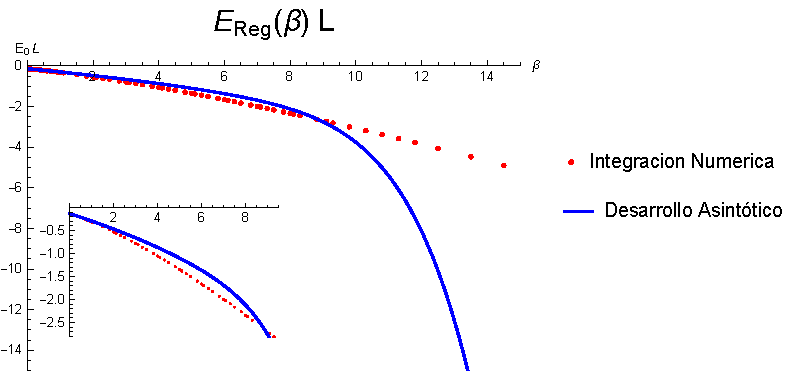
\includegraphics[height=1.3in]{exportar1.pdf}
        \caption{}
        \label{fig.derecha}
    \end{subfigure}%
    ~ 
    \begin{subfigure}[t]{0.5\textwidth}
        \centering
        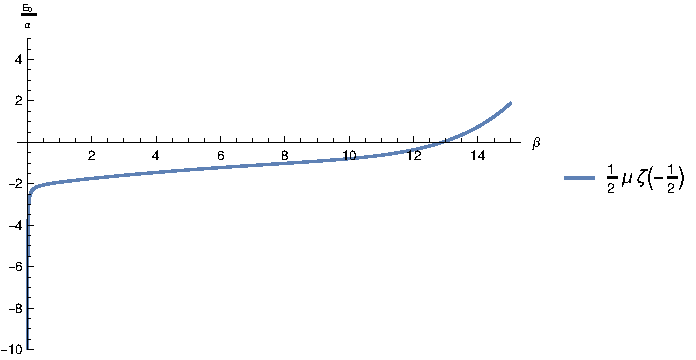
\includegraphics[height=1.3in]{Finita.pdf}
        \caption{}
        \label{fig.izquierda}
    \end{subfigure}
    ~
    \caption{En esta imagen se muestran dos posibles adimensionalizaciones de la energía de vacío, una vez obtenida la curva \ref{fig.izquierda} se pueden generar todas las curvas de la figura \ref{fig:vacios} haciendo los cambios de variables $\beta \rightarrow \alpha L$, $E _0 \rightarrow \frac{E _0}{\alpha}$.}
\label{fig.finitas}
\end{figure*}

\begin{figure*}[t!]
    \centering
    \begin{subfigure}[t]{0.5\textwidth}
        \centering
        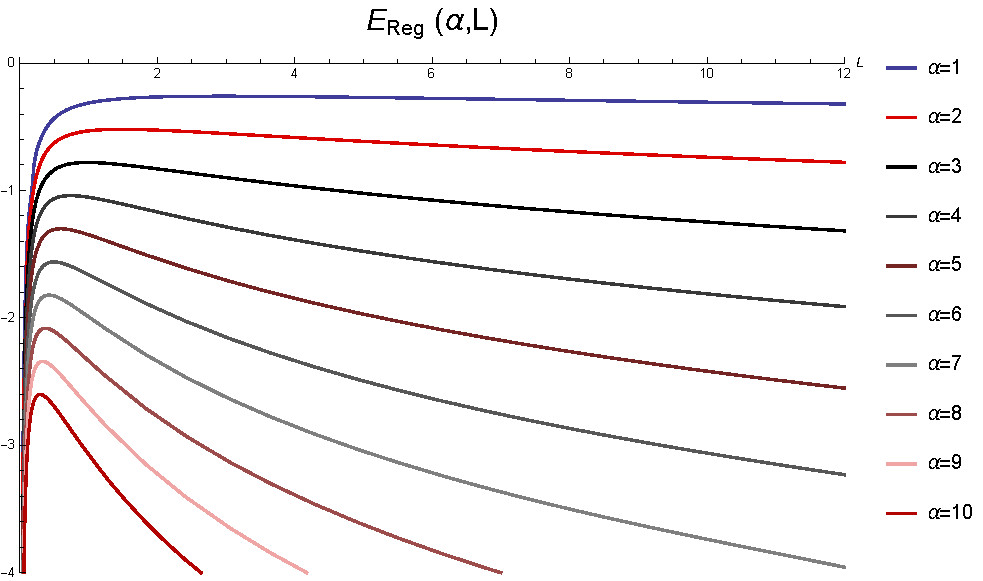
\includegraphics[height=1.45in]{Energias.pdf}
        \caption{}
        \label{fig.izquierda123}
    \end{subfigure}%
    ~ 
    \begin{subfigure}[t]{0.5\textwidth}
        \centering
        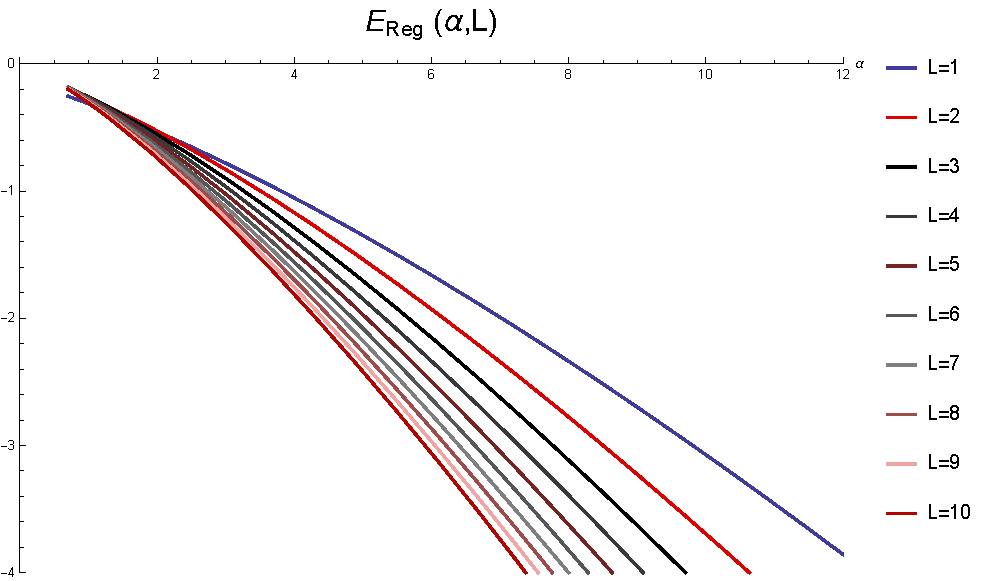
\includegraphics[height=1.45in]{Ls.pdf}
        \caption{}
%        \label{fig.derecha}
    \end{subfigure}
    \caption{En esta imagen se puede observar la dependencia de la energía de Casimir $E _0$ para distintos valores de $\alpha$ y $L$, puede verse en \ref{fig.izquierda123} que a medida que incrementa $\alpha$ la energía de vacío posee un máximo local mas abrupto.}
\label{fig:vacios}
\end{figure*}

\subsection{Integral compleja}\label{sec.finita.compleja}

En la sección \ref{sec.complejo} se mostró que la función $\zeta (s)$ puede representarse mediante una integral en el plano complejo, junto con posibles caminos de integración en la figura \ref{fig:contorno}. En los capítulos anteriores \ref{cap.sencillos}  y \ref{cap.singular} se utilizó el contorno \ref{fig.medio} para obtener la estructura de polos, en este capítulo se utilizará el contorno \ref{fig.derecha.derecha} para obtener tanto los polos como la parte finita  de  $\zeta \left( - \frac{1}{2} \right)$.

A diferencia de la seccion \ref{seq.2.com} donde se utilizó la función $M (\lambda )$ en vez de $F _1 ^{1} \left( 1+\frac{ \alpha}{2 \lambda i },2,2 i \lambda x \right)$ para calcular $\zeta (s)$ dado que ambas funciones poseen los mismos ceros, aquí se utilizará 
$F _1 ^{1} \left( 1+\frac{ \alpha}{2 \lambda i },2,2 i \lambda x \right)$, quedando la función $\zeta$ determinada por
\begin{equation}
	\zeta (s) = 
	\frac{1}{2 \pi i} \int _{\mathcal{C}} 
						\left( \frac{\lambda}{\mu} \right) ^{-2s}
						\partial _ \lambda 
						\log F _1 ^{1} 
						\left( 1+\frac{ \alpha}{2 \lambda i },
							2,2 i \lambda x 
							\right)												
						d \lambda
	\, .
\end{equation}
Utilizando las variables adimensionales $\beta = \alpha L$ y  $\rho = \lambda L$ la ecuación anterior puede reescribirse de la forma
\begin{align}
\label{eq.ultima.int}
	\zeta (s) =& 
	\frac{\left(L \mu \right)^{2s}}{2 \pi i} \int _{\mathcal{C}} 
	f (\rho , \beta) \rho ^{-2s} d \rho 
\, ,
\end{align}
donde $f( \rho, \beta)$ está dada por
\begin{align}
f(\rho, \beta) =& 	
i
\frac{
		\left(1 + \frac{ \beta}{2 i \rho} \right) 
		F _1 ^1 
			\left( 2 + \frac{ \beta}{2 i \rho} ,3 ,2 i \rho \right)
		+ \left( \frac{\beta				
				}
				{2 \rho ^2 } 
				\right)
				( F _{1} ^1 ) ^{(1,0,0)}
				\left( 1 + \frac{\beta}{2 i \rho} ,2 ,2 i \rho
						\right)
		}
		{F _1 ^1 \left( 1 + \frac{\beta}{2 i \rho},2,2 i \rho \right)} 
\, ,	
\nonumber
\end{align}
donde $( F _{1} ^1 ) ^{(1,0,0)} (a,b,z)$ significa $ \partial _a F _{1} ^1  (a,b,z)$.


Utilizando el camino de integración \ref{fig.derecha.derecha}, la integral \ref{eq.ultima.int} puede reescribirse como suma de cuatro integrales
\begin{align}
\label{eq.zeta.completa.2}
	\zeta (s) 
&	
	= 
\\
\nonumber
&
- \frac{L ^{2s}}{2 \pi } 
\Bigg(	  e ^{- i \pi s} \int _0 ^{C _0}
			f (i t,\beta )
			t ^{-2s}  dt 
		+ e ^{- i \pi s} \int _{C _0} ^{\infty}
			f (i t,\beta )
			t ^{-2s}  dt 
\\
\nonumber
&
		+ e ^{i \pi s} \int _{0} ^{C _0} 
			f (-i t,\beta )
			t ^{-2s}  dt 
		+ e ^{i \pi s} \int _{C _0} ^{\infty}
			f (-i t,\beta )
			t ^{-2s}  dt 
	\Bigg)
\, .
\end{align}
Donde la primer integral del segundo y tercer renglón pueden calcularse de manera numérica en $s= -\frac{1}{2}$ dado son convergentes. Las otras dos integrales contienen los polos de $\zeta \left(- \frac{1}{2} \right)$ calculados en la ecuación (\ref{eq.result.zeta.c}), para calcular la parte finita de estas ultimas se utiliza el desarrollo \eqref{eq.completa} obteniendo
\[ 
f   ( i t ,\beta )=
\begin{cases} 
	  f _{+} ( t, \beta) = 
	  i  \left(
			\frac{1}{t} - \frac{\beta}{2 t ^2 } + \frac{\beta}{2 t^2}
			\log (2 t) + \frac{\beta \gamma}{2 t^2} 
			\right) + O (t ^{-3})
\\
	  f _{-} ( t, \beta) =
      i  \left(
			- \frac{1}{t} + \frac{\beta}{2 t ^2 } - \frac{\beta}{2 t^2}
			\log (2 t) - \frac{\beta \gamma}{2 t^2} +2
			\right) + O (t ^{-3})
   \end{cases}   
\]
Donde $f (\pm i t ) = f _{\pm} (t) $.
Utilizando este desarrollo las ultimas dos integrales pueden expresarse
\begin{align}
\nonumber
	\int _{C _0} ^{\infty}
			f (i t,\beta )
			t ^{-2s}  dt =& 
	\int _{C _0} ^{\infty}
		\left(
			f (it, \beta) - f _{+} (t, \beta )			
				\right) t ^{-2s} dt 
\label{eq.arriba1}
\\ &+ 
	\int _{C _0} ^{\infty}
			f _{+} ( t, \beta)
			 t ^{-2s} dt  \\
\nonumber
	\int _{C _0} ^{\infty}
			f (-i t,\beta )
			t ^{-2s}  dt 
=& 
	\int _{C _0} ^{\infty}
		\left(
			f (-it, \beta) - f _{-} (t, \beta )			
				\right) t ^{-2s} dt 
	\\ &+ 
\label{eq.arriba2}
	\int _{C _0} ^{\infty}
			f _{-} ( t, \beta)
			 t ^{-2s} dt
\, .
\end{align}
Donde las integrales en las que se sustrajo $f _{+},f_ {-}$ pueden integrarse numéricamente en $s=- \frac{1}{2}$ dado que son convergentes. 
Las contribuciones divergentes están dadas por
\begin{align}
\label{arriba}
&
	\int _{C _0} ^{\infty}
			f _{+} (t, \beta )			
			 t ^{-2s} dt =  
	O \left( s + \frac{1}{2} \right)
\\[5pt]
\nonumber			
&+
	i \left(- C _0 
		    - \frac{\beta \log C_0 (\gamma + \log 2 - 1 ) 
		    		}{2} 
		    - \frac{\beta \log ^2 C _0}{4}
		    + \frac{\beta ( \gamma + \log 2 -1 )}{4 (s + 1/2)} 
		    + \frac{\beta}{8 (s + \frac{1}{2}) ^2}
					\right)
\\[5pt]
\label{abajo}
&
	\int _{C _0} ^{\infty}
			f _{-} ( t, \beta)
			 t ^{-2s} dt =
	O \left(s + \frac{1}{2} \right)
\\[5pt]
\nonumber
&+
	i \left(C _0 
			- C _0 ^2
		    + \frac{\beta \log C_0 (\gamma + \log 2 - 1 ) 
		    		}{2} 
		    + \frac{\beta \log ^2 C _0}{4}
		    - \frac{\beta ( \gamma + \log 2 -1 )}{4 (s + 1/2)} 
		    - \frac{\beta}{8 (s + \frac{1}{2}) ^2}
					\right)
\end{align}
Utilizando las ecuaciones (\ref{abajo},\ref{arriba},\ref{eq.arriba2},\ref{eq.arriba1}) en (\ref{eq.zeta.completa.2}) se obtiene
\begin{align}
\zeta \left( - \frac{1}{2}  + \epsilon \right) &=
- \frac{i}{2 \pi L \mu} 
\Bigg(	  
		 \int _{C _0} ^{\infty}
			\left(
					f (i t,\beta )
					- f (-i t,\beta )
					- f _{+} (t) 
					+ f _{-} (t)
					\right)
			t   dt   \nonumber
\\ \nonumber
&+
		 \int _{- C _0} ^{C _0}
			f (i t,\beta )
			t   dt 	
	\Bigg)
\\ \nonumber
&
	- \frac{\beta \log ^2 C _0}{4 \pi L \mu}
	- \frac{\beta \log C _0 (\gamma + \log 2 -1 )}{2 \pi L \mu} 
	- \frac{16 C_0 - 8 C _0 ^2 + \pi ^2 \beta}{16 \pi L \mu}
\\ \nonumber
&
	+\frac{\beta \log ^2 (L \mu )}{4 \pi L \mu} 
	+ \frac{\beta \log  (L \mu) (\gamma + \log 2 -1)}{2 \pi L \mu}
\\ 
&	+ \frac{\beta}
		 {8 \pi L \mu  \epsilon ^2} +
	\frac{\beta (\gamma + \log (2 L \mu) -1 ) }
		 {4 \pi L \mu  \epsilon } 
\, .
\end{align}
Donde en la última linea están los polos que coinciden con lo calculado anteriormente en (\ref{eq.zeta.final},\ref{eq.result.zeta.c} y\ref{eq.res.1}), en la penultima linea se encuentra la dependencia no trivial con la escala $\log (L \mu)$ que coincide con la calculada con el método anterior en la ecuación (\ref{eq.zeta.final}).

Utilizando este resultado se obtiene para la energía de vacío
\begin{align}
\label{eq.vacio.completa.finita}
\nonumber
	E _0 (\epsilon )&=  
		\frac{1}{4 \pi i L} 
		\left(
			\int _{-C _0} ^{C _0} f (i t) t dt
			+ \int _{C _0} ^{\infty}  \left( f(i t) - f(-i t) - f _{+} (t) + f _{-} (t) \right) t dt
			\right) 
\\ \nonumber &
	- \frac{\beta \log ^2 (C _0) }{8 \pi L}
	-\frac{\beta \log (C _0) (\gamma -1 + \log 2  )}{4 \pi L}
	+ \frac{C _0 ^2}{4 \pi L}
	- \frac{C _0}{2 \pi L}
	- \frac{\pi \beta}{32 L}
\\ \nonumber &
	+ \frac{\beta \log ^2 L \mu}{8 \pi L}
	+ \frac{\beta (\gamma -1 + \log 2  )  \log L \mu}{4 \pi L}
\\ &
	+ \frac{\beta}{16 \pi L \epsilon ^2}
	+ \frac{\beta (\gamma -1 + \log 2 L \mu )}{8  \pi L \epsilon }
	\, .
\end{align}


\subsection{Comparaciones}

Al momento de graficar las energías de vacío se definio la Energía Regularizada $E _{Reg}$ en las ecuaciones \eqref{integral.ante} y \eqref{integral.ultima}, lo que corresponde tomar $\mu L = 1$ en     \eqref{energia.vacio.final} y \eqref{eq.vacio.completa.finita} respectivamente, de manera que la energía de vacío no dependa de la escala $\mu$.
\begin{align}
\nonumber
&
	\frac{E_ {Reg} ( \beta )}{\alpha}  =
	\frac{ \log ^2 \left( \frac{ 1 }{\pi} \right)}{8 \pi}  +
		\frac{ 
			 \log \left( \frac{ 1 }{\pi}\right)
				( \log (2 \pi ) + \gamma -1 )}  
			{4 \pi }  
	- \frac{ (\gamma + \log (2 \pi ) )}{4 \pi}
\\[5pt]
&
+
	\frac{\pi}{2 \beta}  
			\left(
				- \frac{1}{12} +
				\frac{\beta}{2 \pi ^2} 
				\left(
					\gamma \log (2 \pi)
					+ \gamma _1
					\right) +
								\frac{\gamma ^2 \beta }{2 \pi ^2} +
								\frac{1}{\pi} \sum _{p=2} ^{\infty}
								a_p \zeta (p) 
							\right) 
\, .
\label{integral.ante}
\end{align}
\begin{align}
\nonumber
&
	\frac{E _{Reg} ( \beta ) }{\alpha} =  
		\frac{1}{4 \pi i L} 
		\left(
			\int _{-C _0} ^{C _0} f (i t) t dt
			+ \int _{C _0} ^{\infty}  \left( f(i t) - f(-i t) - f _{+} (t) + f _{-} (t) \right) t dt
			\right) 
\\  &
	- \frac{\beta \log ^2 (C _0) }{8 \pi L}
	-\frac{\beta \log (C _0) (\gamma -1 + \log 2  )}{4 \pi L}
	+ \frac{C _0 ^2}{4 \pi L}
	- \frac{C _0}{2 \pi L}
	- \frac{\pi \beta}{32 L}
	\, .
\label{integral.ultima}
\end{align}

En la figura \ref{fig.finitas} se muestran las energías de vacío adimensionalizacionalizadas de la forma $\frac{E _{Reg}}{\alpha}$ y $E _{Reg} L$. En el rango $0 < \beta < 2$ las curvas se solapan perfectamente, en el intervalo $2 < \beta < 8$ puede observarse una ligera diferenicia entre ambas curvas (lo cual se espera que al aumentar la cantidad de términos $a _p$ disminuya), luego a partir de $10 < \beta$ el método analítico  deja de converger y empieza a exibir un crecimiento polinómico.

En la fígura \ref{fig:vacios} se encuentra graficada la energía de vacio para distintos valores de $\alpha$ y $\beta$, generadas a partir de la interpolacion de los puntos obtenidos con el método integral que se presenta en la figura \ref{fig.finitas}. En esta figura puede observarse que la energía de vacío posee un máximo local alrededor de $\alpha L \sim 0.2$ el cual se hace mas pronunciado al aumentar $\alpha$, este punto determina una región donde la energía de vacío pasa de ser atractiva a repulsiva, lo cual ocurre independientemente de cuan pequeño sea $\alpha$.

